%-----------------------------------
% Define document and include general packages
%-----------------------------------
% Tabellen- und Abbildungsverzeichnis stehen normalerweise nicht im
% Inhaltsverzeichnis. Gleiches gilt für das Abkürzungsverzeichnis (siehe unten).
% Manche Dozenten bemängeln das. Die Optionen 'listof=totoc,bibliography=totoc'
% geben das Tabellen- und Abbildungsverzeichnis im Inhaltsverzeichnis (toc=Table
% of Content) aus.
% Da es aber verschiedene Regelungen je nach Dozent geben kann, werden hier
% beide Varianten dargestellt.
\documentclass[12pt,oneside,titlepage,listof=totoc,bibliography=totoc]{scrartcl}
%\documentclass[12pt,oneside,titlepage]{scrartcl}

%-----------------------------------
% Dokumentensprache
%-----------------------------------
%\def\FOMEN{}% Auskommentieren um die Dokumentensprache auf englisch zu ändern
\newif\ifde
\newif\ifen

%-----------------------------------
% Meta informationen
%-----------------------------------
%-----------------------------------
% Meta Informationen zur Arbeit
%-----------------------------------

% Autor
\newcommand{\myAutor}{Julian Türner}

% Adresse
\newcommand{\myAdresse}{Heidestra\ss e 17 \\ \> \> \> 51147 Köln}

% Titel der Arbeit
\newcommand{\myTitel}{Untersuchung der Navigation eines autonomen Fahrzeugs im Gelände: Ein Experiment mit bildbasierter Routenführung (Exposé)}

% Betreuer
\newcommand{\myBetreuer}{Dr.-Ing. Nadine Neumann}

% Lehrveranstaltung
\newcommand{\myLehrveranstaltung}{Vorbereitungsseminar zur Bachelor-Thesis}

% Matrikelnummer
\newcommand{\myMatrikelNr}{581388}

% Ort
\newcommand{\myOrt}{München}

% Datum der Abgabe
\newcommand{\myAbgabeDatum}{\today}

% Semesterzahl
\newcommand{\mySemesterZahl}{6}

% Name der Hochschule
\newcommand{\myHochschulName}{FOM Hochschule für Oekonomie \& Management}

% Standort der Hochschule
\newcommand{\myHochschulStandort}{München}

% Studiengang
\newcommand{\myStudiengang}{Informatik}

% Art der Arbeit
\newcommand{\myThesisArt}{Exposé zur Bachelor-Thesis}

% Zu erlangender akademische Grad
\newcommand{\myAkademischerGrad}{Bachelor of Science (B.Sc.)}

% Firma
\newcommand{\myFirma}{Mustermann GmbH}


\ifdefined\FOMEN
%Englisch
\entrue
\usepackage[english]{babel}
\else
%Deutsch
\detrue
\usepackage[ngerman]{babel}
\fi


\newcommand{\langde}[1]{%
   \ifde\selectlanguage{ngerman}#1\fi}
\newcommand{\langen}[1]{%
   \ifen\selectlanguage{english}#1\fi}
\usepackage[utf8]{luainputenc}
\langde{\usepackage[babel,german=quotes]{csquotes}}
\langen{\usepackage[babel,english=british]{csquotes}}
\usepackage[T1]{fontenc}
\usepackage{fancyhdr}
\usepackage{fancybox}
\usepackage[a4paper, left=4cm, right=2cm, top=4cm, bottom=2cm]{geometry}
\usepackage{graphicx}
\usepackage{colortbl}
\usepackage[capposition=top]{floatrow}
\usepackage{array}
\usepackage{float}      %Positionierung von Abb. und Tabellen mit [H] erzwingen
\usepackage{footnote}
% Darstellung der Beschriftung von Tabellen und Abbildungen (Leitfaden S. 44)
% singlelinecheck=false: macht die Caption linksbündig (statt zentriert)
% labelfont auf fett: (Tabelle x.y:, Abbildung: x.y)
% font auf fett: eigentliche Bezeichnung der Abbildung oder Tabelle
% Fettschrift laut Leitfaden 2018 S. 45
\usepackage[singlelinecheck=false, labelfont=bf, font=bf]{caption}
\usepackage{caption}
\usepackage{enumitem}
\usepackage{amssymb}
\usepackage{mathptmx}
%\usepackage{minted} %Kann für schöneres Syntax Highlighting genutzt werden. ACHTUNG: Python muss installiert sein.
\usepackage[scaled=0.9]{helvet} % Behebt, zusammen mit Package courier, pixelige Überschriften. Ist, zusammen mit mathptx, dem times-Package vorzuziehen. Details: https://latex-kurs.de/fragen/schriftarten/Times_New_Roman.html
\usepackage{courier}
\usepackage{amsmath}
\usepackage[table]{xcolor}
\usepackage{marvosym}			% Verwendung von Symbolen, z.B. perfektes Eurozeichen

\renewcommand\familydefault{\sfdefault}
\usepackage{ragged2e}

% Mehrere Fussnoten nacheinander mit Komma separiert
\usepackage[hang,multiple]{footmisc}
\setlength{\footnotemargin}{1em}

% todo Aufgaben als Kommentare verfassen für verschiedene Editoren
\usepackage{todonotes}

% Verhindert, dass nur eine Zeile auf der nächsten Seite steht
\setlength{\marginparwidth}{2cm}
\usepackage[all]{nowidow}

%-----------------------------------
% Farbdefinitionen
%-----------------------------------
\definecolor{darkblack}{rgb}{0,0,0}
\definecolor{dunkelgrau}{rgb}{0.8,0.8,0.8}
\definecolor{hellgrau}{rgb}{0.0,0.7,0.99}
\definecolor{mauve}{rgb}{0.58,0,0.82}
\definecolor{dkgreen}{rgb}{0,0.6,0}

%-----------------------------------
% Pakete für Tabellen
%-----------------------------------
\usepackage{epstopdf}
\usepackage{nicefrac} % Brüche
\usepackage{multirow}
\usepackage{rotating} % vertikal schreiben
\usepackage{mdwlist}
\usepackage{tabularx}% für Breitenangabe

%-----------------------------------
% sauber formatierter Quelltext
%-----------------------------------
\usepackage{listings}
% JavaScript als Sprache definieren:
\lstdefinelanguage{JavaScript}{
	keywords={break, super, case, extends, switch, catch, finally, for, const, function, try, continue, if, typeof, debugger, var, default, in, void, delete, instanceof, while, do, new, with, else, return, yield, enum, let, await},
	keywordstyle=\color{blue}\bfseries,
	ndkeywords={class, export, boolean, throw, implements, import, this, interface, package, private, protected, public, static},
	ndkeywordstyle=\color{darkgray}\bfseries,
	identifierstyle=\color{black},
	sensitive=false,
	comment=[l]{//},
	morecomment=[s]{/*}{*/},
	commentstyle=\color{purple}\ttfamily,
	stringstyle=\color{red}\ttfamily,
	morestring=[b]',
	morestring=[b]"
}

\lstset{
	%language=JavaScript,
	numbers=left,
	numberstyle=\tiny,
	numbersep=5pt,
	breaklines=true,
	showstringspaces=false,
	frame=l ,
	xleftmargin=5pt,
	xrightmargin=5pt,
	basicstyle=\ttfamily\scriptsize,
	stepnumber=1,
	keywordstyle=\color{blue},          % keyword style
  	commentstyle=\color{dkgreen},       % comment style
  	stringstyle=\color{mauve}         % string literal style
}

%-----------------------------------
%Literaturverzeichnis Einstellungen
%-----------------------------------

% Biblatex

\usepackage{url}
\urlstyle{same}

%%%% Neuer Leitfaden (2018)
\usepackage[
backend=biber,
style=ieee,
maxcitenames=3,	% mindestens 3 Namen ausgeben bevor et. al. kommt
maxbibnames=999,
date=iso,
seconds=true, %werden nicht verwendet, so werden aber Warnungen unterdrückt.
urldate=iso,
dashed=false,
autocite=inline,
useprefix=true, % 'von' im Namen beachten (beim Anzeigen)
mincrossrefs = 1
]{biblatex}%iso dateformat für YYYY-MM-DD

%weitere Anpassungen für BibLaTex
% \usepackage{xpatch}

\setlength\bibhang{1cm}

%%% Weitere Optionen
%\boolitem[false]{citexref} %Wenn incollection, inbook, inproceedings genutzt wird nicht den zugehörigen parent auch in Literaturverzeichnis aufnehmen

%Aufräumen die Felder werden laut Leitfaden nicht benötigt.
\AtEveryBibitem{%
\ifentrytype{book}{
    \clearfield{issn}%
    \clearfield{doi}%
    \clearfield{isbn}%
    \clearfield{url}
    \clearfield{eprint}
}{}
\ifentrytype{collection}{
  \clearfield{issn}%
  \clearfield{doi}%
  \clearfield{isbn}%
  \clearfield{url}
  \clearfield{eprint}
}{}
\ifentrytype{incollection}{
  \clearfield{issn}%
  \clearfield{doi}%
  \clearfield{isbn}%
  \clearfield{url}
  \clearfield{eprint}
}{}
\ifentrytype{article}{
  \clearfield{issn}%
  \clearfield{doi}%
  \clearfield{isbn}%
  \clearfield{url}
  \clearfield{eprint}
}{}
\ifentrytype{inproceedings}{
  \clearfield{issn}%
  \clearfield{doi}%
  \clearfield{isbn}%
  \clearfield{url}
  \clearfield{eprint}
}{}
}

\renewcommand*{\finentrypunct}{}%Kein Punkt am ende des Literaturverzeichnisses

\renewcommand*{\newunitpunct}{\addcomma\space}
\DeclareDelimFormat[bib,biblist]{nametitledelim}{\addcolon\space}
\DeclareDelimFormat{titleyeardelim}{\newunitpunct}
%Namen kursiv schreiben
\renewcommand*{\mkbibnamefamily}{\mkbibemph}
\renewcommand*{\mkbibnamegiven}{\mkbibemph}
\renewcommand*{\mkbibnamesuffix}{\mkbibemph}
\renewcommand*{\mkbibnameprefix}{\mkbibemph}

% Die Trennung mehrerer Autorennamen erfolgt durch Kommata.
% siehe Beispiele im Leitfaden S. 16
% Die folgende Zeile würde mit Semikolon trennen
%\DeclareDelimFormat{multinamedelim}{\addsemicolon\addspace}

%Delimiter für mehrere und letzten Namen gleich setzen
\DeclareDelimAlias{finalnamedelim}{multinamedelim}

\DeclareNameAlias{default}{family-given}
\DeclareNameAlias{sortname}{default}  %Nach Namen sortieren


\DeclareFieldFormat{editortype}{\mkbibparens{#1}}
\DeclareDelimFormat{editortypedelim}{\addspace}
\DeclareFieldFormat{translatortype}{\mkbibparens{#1}}
\DeclareDelimFormat{translatortypedelim}{\addspace}
\DeclareDelimFormat[bib,biblist]{innametitledelim}{\addcomma\space}

\DeclareFieldFormat*{citetitle}{#1}
\DeclareFieldFormat*{title}{#1}
\DeclareFieldFormat*{booktitle}{#1}
\DeclareFieldFormat*{journaltitle}{#1}

\xpatchbibdriver{online}
  {\usebibmacro{organization+location+date}\newunit\newblock}
  {}
  {}{}

\DeclareFieldFormat[online]{date}{\mkbibparens{#1}}
\DeclareFieldFormat{urltime}{\addspace #1\addspace \langde{Uhr}\langen{MEZ}}
\DeclareFieldFormat{urldate}{%urltime zu urldate hinzufügen
  [\langde{Zugriff}\langen{Access}\addcolon\addspace
  #1\printfield{urltime}]
}
\DeclareFieldFormat[online]{url}{<\url{#1}>}
\renewbibmacro*{url+urldate}{%
  \usebibmacro{url}%
  \ifentrytype{online}
    {\setunit*{\addspace}%
     \iffieldundef{year}
       {\printtext[date]{\langde{keine Datumsangabe}\langen{no Date} }}
       {\usebibmacro{date}}}%
    {}%
  \setunit*{\addspace}%
  \usebibmacro{urldate}
  }

%Verhindern, dass bei mehreren Quellen des gleichen Autors im gleichen Jahr
%Buchstaben nach der Jahreszahl angezeigt werden wenn sich das Keyword in usera unterscheidet.
\DeclareExtradate{
  \scope{
    \field{labelyear}
    \field{year}
    }
    \scope{
      \field{usera}
     }
}

%% Anzeige des Jahres nach dem Stichwort (usera) im Literaturverzeichnis
%% Wenn das Jahr bei Online-Quellen nicht explizit angegeben wurde, wird nach
%% dem Stichwort 'o. J.' ausgegeben. Nach der URL steht dann 'keine
%% Datumsangabe'. Ist das Jahr definiert, wird es an beiden Stellen ausgegeben.
%% Das Zugriffsdatum (urldate) spielt hier keine Rolle.
%% Für Nicht-Online-Quellen wird nichts geändert.
\renewbibmacro*{date+extradate}{%
  \printtext[parens]{%
    \printfield{usera}%
    \setunit{\printdelim{titleyeardelim}}%
    \ifentrytype{online}
       {\setunit*{\addspace\addcomma\addspace}%
         \iffieldundef{year}
           {\bibstring{nodate}}
       {\printlabeldateextra}}%
       {\printlabeldateextra}}}

%% Anzeige des Jahres nach dem Stichwort (usera) in der Fussnote
%% das Stichwort hat der Aufrufer hier schon ausgegeben.
%% siehe auch Kommentar zu: \renewbibmacro*{date+extradate}
\renewbibmacro*{cite:labeldate+extradate}{%
    \ifentrytype{online}
       {\setunit*{\addspace\addcomma\addspace}%
         \iffieldundef{year}
           {\bibstring{nodate}}
       {\printlabeldateextra}}%
       {\printlabeldateextra}}


\DefineBibliographyStrings{german}{
  nodate    = {{}o.\adddot\addspace J\adddot},
  andothers = {et\addabbrvspace al\adddot}
}
\DefineBibliographyStrings{english}{
  nodate    = {{}n.\adddot\addspace d\adddot},
  andothers = {et\addabbrvspace al\adddot}
}
\DeclareSourcemap{
  \maps[datatype=bibtex]{
    \map{
      \step[notfield=translator, final]
      \step[notfield=editor, final]
      \step[fieldset=author, fieldvalue={{{\langde{o\noexpand\adddot\addspace V\noexpand\adddot}\langen{Anon}}}}]
    }
    \map{
      \pernottype{online}
      \step[fieldset=location, fieldvalue={\langde{o\noexpand\adddot\addspace O\noexpand\adddot}\langen{s\noexpand\adddot I\noexpand\adddot}}]
    }
  }
}

\renewbibmacro*{cite}{%
  \iffieldundef{shorthand}
    {\ifthenelse{\ifnameundef{labelname}\OR\iffieldundef{labelyear}}
       {\usebibmacro{cite:label}%
        \setunit{\printdelim{nonametitledelim}}}
       {\printnames{labelname}%
        \setunit{\printdelim{nametitledelim}}}%
     \printfield{usera}%
     \setunit{\printdelim{titleyeardelim}}%
     \usebibmacro{cite:labeldate+extradate}}
    {\usebibmacro{cite:shorthand}}}

    \renewcommand*{\jourvoldelim}{\addcomma\addspace}% Trennung zwischen journalname und Volume. Sonst Space; Laut Leitfaden richtig
    %Aufgrund der Änderung bzgl des Issues 169 in der thesis_main.tex musste ich die Zeile auskommentieren. Konnte aber das Verhalten, dass die Fußnoten grün sind, im nachhinein nicht feststellen.
    %\hypersetup{hidelinks} %sonst sind Fußnoten grün. Dadurch werden Links allerdings nicht mehr farbig dargestellt

\renewbibmacro*{journal+issuetitle}{%
  \usebibmacro{journal}%
  \setunit*{\jourvoldelim}%
  \iffieldundef{series}
    {}
    {\setunit*{\jourserdelim}%
     \printfield{series}%
     \setunit{\servoldelim}}%
  \iffieldundef{volume}
    {}
    {\printfield{volume}}
  \iffieldundef{labelyear}
  {}
  {
  (\thefield{year}) %Ansonsten wird wenn kein Volume angegeben ist ein Komma vorangestellt
  }
  \setunit*{\addcomma\addspace Nr\adddot\addspace}
  \printfield{number}
  \iffieldundef{eid}
  {}
  {\printfield{eid}}
}

% Postnote ist der Text in der zweiten eckigen Klammer bei einem Zitat
% wenn es keinen solchen Eintrag gibt, dann auch nicht ausgeben, z.B. 'o. S.'
% Wenn man das will, kann man das 'o. S.' ja explizit angeben. Andernfalls steht
% sonst auch bei Webseiten 'o. S.' da, was laut Leitfaden nicht ok ist.
\renewbibmacro*{postnote}{%
  \setunit{\postnotedelim}%
  \iffieldundef{postnote}
    {} %{\printtext{\langde{o.S\adddot}\langen{no page number}}}
    {\printfield{postnote}}}

% Abstand bei Änderung Anfangsbuchstabe ca. 1.5 Zeilen
\setlength{\bibinitsep}{0.75cm}

% nur in den Zitaten/Fussnoten den Vornamen abkürzen (nicht im
% Literaturverzeichnis)

\DeclareDelimFormat{nonameyeardelim}{\addcomma\space}
\DeclareDelimFormat{nameyeardelim}{\addcomma\space}

\renewbibmacro*{cite}{%
  \iffieldundef{shorthand}
    {\ifthenelse{\ifciteibid\AND\NOT\iffirstonpage}
       {\usebibmacro{cite:ibid}}
    {\printtext[bibhyperref]{\ifthenelse{\ifnameundef{labelname}\OR\iffieldundef{labelyear}}
       {\usebibmacro{cite:label}%
        \setunit{\printdelim{nonameyeardelim}}}
      {\toggletrue{abx@bool@giveninits}%
        \printnames[family-given]{labelname}%
        \setunit{\printdelim{nameyeardelim}}}%
      \printfield{usera}%
      \setunit{\printdelim{titleyeardelim}}%
     \usebibmacro{cite:labeldate+extradate}}}}
   {\usebibmacro{cite:shorthand}}}

%%%%% Alter Leitfaden. Ggf. Einkommentieren und Bereich hierüber auskommentieren
%\usepackage[
%backend=biber,
%style=numeric,
%citestyle=authoryear,
%url=false,
%isbn=false,
%notetype=footonly,
%hyperref=false,
%sortlocale=de]{biblatex}

%weitere Anpassungen für BibLaTex
%% Opptionen für Biblatex
\ExecuteBibliographyOptions{%
giveninits=false,
isbn=true,
url=true,
doi=false,
eprint=false,
maxbibnames=7, % Alle Autoren (kein et al.)
maxcitenames=2, % et al. ab dem 3. Autor
backref=false, % Rückverweise auf Zitatseiten
bibencoding=utf8, % wenn .bib in utf8, sonst ascii
bibwarn=true, % Warnung bei fehlerhafter bib-Datei
}%

% et al. an Stelle von u.a.
\DefineBibliographyStrings{ngerman}{
   andothers = {{et\,al\adddot}},
}

% Klammern um das Jahr in der Fußnote
\renewbibmacro*{cite:labelyear+extrayear}{%
  \iffieldundef{labelyear}
    {}
    {\printtext[bibhyperref]{%
       \mkbibparens{%
         \printfield{labelyear}%
         \printfield{extrayear}}}}}

\renewbibmacro*{cite:title}{%
  \printtext[bibhyperref]{%
    \printfield[citetitle]{labeltitle}%
    \setunit{\addcomma\space}%
    \printdate}}

\DeclareNameFormat{last-first}{%
  \iffirstinits
    {\usebibmacro{name:family-given}
        {\namepartfamily}
        {\namepartgiveni}
        {\namepartprefix}
        {\namepartsuffix}
    }
    {\usebibmacro{name:family-given}
        {\namepartfamily}
        {\namepartgiven}
        {\namepartprefix}
        {\namepartsuffix}
    }%
  \usebibmacro{name:andothers}}

% Alternative Notation der Fußnoten
% Zeigt sowohl den Nachnamen als auch den Vornamen an
% Beispiel: \fullfootcite[Vgl. ][Seite 5]{Tanenbaum.2003}
\DeclareCiteCommand{\fullfootcite}[\mkbibfootnote]
  {\usebibmacro{prenote}}
  {\usebibmacro{citeindex}%
    \printnames[sortname][1-1]{author}%
    \addspace (\printfield{year})}
  {\addsemicolon\space}
  {\usebibmacro{postnote}}

%Autoren (Nachname, Vorname)
\DeclareNameAlias{default}{family-given}

%Reihenfolge von publisher, year, address verändern
% Achtung, bisher nur für den Typ @book definiert

%% Definiert @Book Eintrag
\DeclareBibliographyDriver{book}{%
  \printnames{author}%
  \newunit\addcolon\space
  \printfield{title}%
  \setunit*{,\space}%
  \printfield{edition}%
  \setunit*{\addcomma\space}%
  \printlist{publisher}%
  \newunit\newblockpunct
  \printlist{location}%
  \setunit*{\space}%
  \printfield{year}%
  \setunit*{,\space}%
  \printfield{isbn}%
  \finentry}

%% Definiert @Online Eintrag
\DeclareBibliographyDriver{online}{%
  \printnames{author}%
  \newunit\newblockpunct
  \printfield{title}%
  \setunit*{,\space}%
  %\newunit\newblock
  \printfield{url}%
  \setunit*{,\space Erscheinungsjahr:\space}%
  \printfield{year}%
  \setunit*{,\space Aufruf am:\space}%
  \printfield{note}%
  \finentry}

%% Definiert @Article Eintrag
\DeclareBibliographyDriver{article}{%
  \printnames{author}%
  \newunit\newblockpunct
  \printfield{title}%
  \setunit*{.\space In:\space}%
  %\newunit\newblock
  \usebibmacro{journal}%
  \setunit*{\space (}%
  \printfield{year}\newunit{)}%
  \finentry}

%% Definiert @InProceedings Eintrag
\DeclareBibliographyDriver{inproceedings}{%
	\printnames{author}%
	\setunit*{,\space (}%
	\printfield{year}\newunit{)}%
	\newunit\newblockpunct
	\printfield{title}%
	\setunit*{\space}%
	\usebibmacro{booktitle}%
	\setunit*{,\space}%
	\printfield{isbn}%
	\setunit*{,\space}%
	\printfield{doi}%
	\finentry}

%Doppelpunkt nach dem letzten Autor
\renewcommand*{\labelnamepunct}{\addcolon\addspace }

%Komma an Stelle des Punktes
\renewcommand*{\newunitpunct}{\addcomma\space}

%Autoren durch Semikolon trennen
\newcommand*{\bibmultinamedelim}{\addsemicolon\space}%
\newcommand*{\bibfinalnamedelim}{\addsemicolon\space}%
\AtBeginBibliography{%
  \let\multinamedelim\bibmultinamedelim
  \let\finalnamedelim\bibfinalnamedelim
}

%Titel nicht kursiv anzeigen
\DeclareFieldFormat{title}{#1\isdot}


%%%% Ende Alter Leitfaden

%Bib-Datei einbinden
\addbibresource{literatur/literatur.bib}

% Zeilenabstand im Literaturverzeichnis ist Einzeilig
% siehe Leitfaden S. 14
\AtBeginBibliography{\singlespacing}

%-----------------------------------
% Silbentrennung
%-----------------------------------
\usepackage{hyphsubst}
\HyphSubstIfExists{ngerman-x-latest}{%
\HyphSubstLet{ngerman}{ngerman-x-latest}}{}

%-----------------------------------
% Pfad fuer Abbildungen
%-----------------------------------
\graphicspath{{./}{./abbildungen/}}

%-----------------------------------
% Weitere Ebene einfügen
%-----------------------------------
\usepackage{titletoc}

\makeatletter

% Setze die Tiefe des Inhaltsverzeichnis auf 4 Ebenen
% Damit erscheinen \paragraph-Sektionen auch im Inhaltsverzeichnis
\setcounter{secnumdepth}{4}
\setcounter{tocdepth}{4}

% Fuege Abstand nach unten wie in einer normalen \section hinzu
% Andernfalls haette \paragraph keinen Zeilenumbruch
% Der Zeilenumbruch koennte mit einer leeren \mbox{} ersetzt werden
% Jedoch klebt dann der Text relativ nah an der Ueberschrift
\renewcommand{\paragraph}{%
  \@startsection{paragraph}{4}%
  {\z@}{3.25ex \@plus 1ex \@minus .2ex}{1.5ex plus 0.2ex}%
  {\normalfont\normalsize\bfseries\sffamily}%
}

\makeatother


%-----------------------------------
% Paket für die Nutzung von Anhängen
%-----------------------------------
\usepackage{appendix}

%-----------------------------------
% Zeilenabstand 1,5-zeilig
%-----------------------------------
\usepackage{setspace}
\onehalfspacing

%-----------------------------------
% Absätze durch eine neue Zeile
%-----------------------------------
\setlength{\parindent}{0mm}
\setlength{\parskip}{0.8em plus 0.5em minus 0.3em}

\sloppy					%Abstände variieren
\pagestyle{headings}

%----------------------------------
% Präfix in das Abbildungs- und Tabellenverzeichnis aufnehmen, statt nur der Nummerierung (siehe Issue #206).
%----------------------------------
\KOMAoption{listof}{entryprefix} % Siehe KOMA-Script Doku v3.28 S.153
\BeforeStartingTOC[lof]{\renewcommand*\autodot{:}} % Für den Doppelpunkt hinter Präfix im Abbildungsverzeichnis
\BeforeStartingTOC[lot]{\renewcommand*\autodot{:}} % Für den Doppelpunkt hinter Präfix im Tabellenverzeichnis

%-----------------------------------
% Abkürzungsverzeichnis
%-----------------------------------
\usepackage[printonlyused]{acronym}

%-----------------------------------
% Symbolverzeichnis
%-----------------------------------
% Quelle: https://www.namsu.de/Extra/pakete/Listofsymbols.pdf
\usepackage[final]{listofsymbols}

%-----------------------------------
% Glossar
%-----------------------------------
\usepackage{glossaries}
\glstoctrue %Auskommentieren, damit das Glossar nicht im Inhaltsverzeichnis angezeigt wird.
\makenoidxglossaries
\newglossaryentry{glossar}{name={Glossar},description={In einem Glossar werden Fachbegriffe und Fremdwörter mit ihren Erklärungen gesammelt.}}
\newglossaryentry{glossaries}{name={Glossaries},description={Glossaries ist ein Paket was einen im Rahmen von LaTeX bei der Erstellung eines Glossar unterstützt.}}
\newglossaryentry{UGV}
{
    name=Unmanned Ground Vehicle,
    description={Ein unbemanntes Bodenfahrzeug, das autonom oder ferngesteuert betrieben wird, typischerweise für militärische oder zivile Anwendungen}
}

\newglossaryentry{UAV}
{
    name=Unmanned Air Vehicle,
    description={Ein unbemanntes Luftfahrzeug, das autonom oder ferngesteuert betrieben wird, oft für Aufklärungs- oder Überwachungsmissionen}
}

\newglossaryentry{CNN}
{
    name=Convolutional Neural Network,
    description={Ein tiefes neuronales Netzwerk, das speziell für die Verarbeitung von Bilddaten entwickelt wurde}
}

\newglossaryentry{IMUGS}
{
    name=Integrated Modular Unmanned Ground System,
    description={Ein Projekt zur Entwicklung modularer unbemannter Bodensysteme, das von der EU finanziert wird}
}

\newglossaryentry{SLAM}
{
    name=Simultaneous Localization and Mapping,
    description={Ein Algorithmus, der es einem mobilen Roboter ermöglicht, eine Karte seiner Umgebung zu erstellen und gleichzeitig seine Position in dieser Karte zu bestimmen}
}

\newglossaryentry{OpenCV}
{
    name=OpenCV,
    description={Eine Open-Source-Bibliothek für Computer Vision und maschinelles Lernen, die zur Bildverarbeitung und -analyse verwendet wird}
}

\newglossaryentry{AirSim}
{
    name=AirSim,
    description={Ein hochrealistischer Simulator für autonome Fahrzeuge und Drohnen, der auf der Unreal Engine basiert}
}

\newglossaryentry{Unreal Engine}
{
    name=Unreal Engine,
    description={Eine von Epic Games entwickelte Game-Engine, die häufig für die Entwicklung von Videospielen und Simulationen verwendet wird}
}

\newglossaryentry{BirdView}
{
    name=BirdView,
    description={Eine Perspektive, die das Gelände aus einer erhöhten Position zeigt, ähnlich der Ansicht eines Vogels}
}

\newglossaryentry{Feature Matching}
{
    name=Feature Matching,
    description={Ein Verfahren in der Bildverarbeitung, bei dem markante Merkmale in verschiedenen Bildern erkannt und miteinander verglichen werden}
}
\newglossaryentry{LIDAR}
{
    name=LIDAR,
    description={Ein Verfahren zur optischen Abstandsmessung, das auf der Aussendung und dem Empfang von Lichtimpulsen basiert. Es wird häufig in autonomen Fahrzeugen verwendet, um die Umgebung in 3D zu erfassen}
}

\newglossaryentry{GPS-denied}
{
    name=GPS-denied,
    description={Bezeichnet Umgebungen, in denen das \ac{GPS} aufgrund von Störungen, Abschattungen oder anderen Faktoren nicht verfügbar oder stark eingeschränkt ist, was eine alternative Navigationstechnologie erfordert}
}



%-----------------------------------
% PDF Meta Daten setzen
%-----------------------------------
\usepackage[hyperfootnotes=false]{hyperref} %hyperfootnotes=false deaktiviert die Verlinkung der Fußnote. Ansonsten inkompaibel zum Paket "footmisc"
% Behebt die falsche Darstellung der Lesezeichen in PDF-Dateien, welche eine Übersetzung besitzen
% siehe Issue 149
\makeatletter
\pdfstringdefDisableCommands{\let\selectlanguage\@gobble}
\makeatother

\hypersetup{
    pdfinfo={
        Title={\myTitel},
        Subject={\myStudiengang},
        Author={\myAutor},
        Build=1.1
    }
}

%-----------------------------------
% PlantUML
%-----------------------------------
%\usepackage{plantuml}

%-----------------------------------
% Umlaute in Code korrekt darstellen
% siehe auch: https://en.wikibooks.org/wiki/LaTeX/Source_Code_Listings
%-----------------------------------
\lstset{literate=
	{á}{{\'a}}1 {é}{{\'e}}1 {í}{{\'i}}1 {ó}{{\'o}}1 {ú}{{\'u}}1
	{Á}{{\'A}}1 {É}{{\'E}}1 {Í}{{\'I}}1 {Ó}{{\'O}}1 {Ú}{{\'U}}1
	{à}{{\`a}}1 {è}{{\`e}}1 {ì}{{\`i}}1 {ò}{{\`o}}1 {ù}{{\`u}}1
	{À}{{\`A}}1 {È}{{\'E}}1 {Ì}{{\`I}}1 {Ò}{{\`O}}1 {Ù}{{\`U}}1
	{ä}{{\"a}}1 {ë}{{\"e}}1 {ï}{{\"i}}1 {ö}{{\"o}}1 {ü}{{\"u}}1
	{Ä}{{\"A}}1 {Ë}{{\"E}}1 {Ï}{{\"I}}1 {Ö}{{\"O}}1 {Ü}{{\"U}}1
	{â}{{\^a}}1 {ê}{{\^e}}1 {î}{{\^i}}1 {ô}{{\^o}}1 {û}{{\^u}}1
	{Â}{{\^A}}1 {Ê}{{\^E}}1 {Î}{{\^I}}1 {Ô}{{\^O}}1 {Û}{{\^U}}1
	{œ}{{\oe}}1 {Œ}{{\OE}}1 {æ}{{\ae}}1 {Æ}{{\AE}}1 {ß}{{\ss}}1
	{ű}{{\H{u}}}1 {Ű}{{\H{U}}}1 {ő}{{\H{o}}}1 {Ő}{{\H{O}}}1
	{ç}{{\c c}}1 {Ç}{{\c C}}1 {ø}{{\o}}1 {å}{{\r a}}1 {Å}{{\r A}}1
	{€}{{\EUR}}1 {£}{{\pounds}}1 {„}{{\glqq{}}}1
}

%-----------------------------------
% Kopfbereich / Header definieren
%-----------------------------------
\pagestyle{fancy}
\fancyhf{}
% Seitenzahl oben, mittig, mit Strichen beidseits
% \fancyhead[C]{-\ \thepage\ -}

% Seitenzahl oben, mittig, entsprechend Leitfaden ohne Striche beidseits
\fancyhead[C]{\thepage}
%\fancyhead[L]{\leftmark}							% kein Footer vorhanden
% Waagerechte Linie unterhalb des Kopfbereiches anzeigen. Laut Leitfaden ist
% diese Linie nicht erforderlich. Ihre Breite kann daher auf 0pt gesetzt werden.
\renewcommand{\headrulewidth}{0.4pt}
%\renewcommand{\headrulewidth}{0pt}

%-----------------------------------
% Damit die hochgestellten Zahlen auch auf die Fußnote verlinkt sind (siehe Issue 169)
%-----------------------------------
\hypersetup{colorlinks=true, breaklinks=true, linkcolor=darkblack, citecolor=darkblack, menucolor=darkblack, urlcolor=darkblack, linktoc=all, bookmarksnumbered=false, pdfpagemode=UseOutlines, pdftoolbar=true}
\urlstyle{same}%gleiche Schriftart für den Link wie für den Text

%-----------------------------------
% Start the document here:
%-----------------------------------
\begin{document}

\pagenumbering{Roman}								% Seitennumerierung auf römisch umstellen
\newcolumntype{C}{>{\centering\arraybackslash}X}	% Neuer Tabellen-Spalten-Typ:
%Zentriert und umbrechbar

%-----------------------------------
% Textcommands
%-----------------------------------
%----------------------------------
%  TextCommands
%----------------------------------
%
%
%
%
%----------------------------------
%  common textCommands
%----------------------------------
% Information: OL bedeutet ohne Leerzeichen. Damit man dieses Command z. B. vor einem Komma oder vor einem anderen Zeichen verwenden kann. Dies ist ein Best-Practis von mir und hat sich sehr bewehrt.
% Allgemein hat es sich bewert alle Wörter die man häufig schreibt und wahrscheinlich falsch oder unterscheidlich schreibt, als Textcommand zu hinterlegen.
% 
%
%
\renewcommand{\symheadingname}{\langde{Symbolverzeichnis}\langen{List of Symbols}}
\newcommand{\abbreHeadingName}{\langde{Abkürzungsverzeichnis}\langen{List of Abbreviations}}
\newcommand{\headingNameInternetSources}{\langde{Internetquellen}\langen{Internet sources}}
\newcommand{\headingNameAiSources}{\langde{KI-Hilfsmittelverzeichnis}\langen{AI sources}}
\newcommand{\AppendixName}{\langde{Anhang}\langen{Appendix}}
\newcommand{\vglf}{\langde{Vgl.}\langen{compare}}
\newcommand{\pagef}{\langde{S. }\langen{p. }}
\newcommand{\os}{\mbox{o. S}}
\newcommand{\ojol}{\mbox{o. J.}}
\newcommand{\oj}{\ojol\ }
\newcommand{\og}{\mbox{o. g.}\ }
\newcommand{\ua}{\mbox{u. a.}\ }
\newcommand{\dah}{\mbox{d. h.}\ }
\newcommand{\zbol}{\mbox{z. B.}}
\newcommand{\zb}{\zbol\ }
\newcommand{\uamol}{unter anderem}
\newcommand{\uam}{\uamol\ }
\newcommand{\uanol}{unter anderen}%mit Leerzeichen
\newcommand{\uan}{\uanol\ }%mit Leerzeichen
\newcommand{\abbol}{Ab"-bil"-dung}
\newcommand{\abb}{\abbol\ }
\newcommand{\tabol}{Tabelle}
\newcommand{\tab}{\tabol\ }
\newcommand{\ggfol}{ggf.}
\newcommand{\ggf}{\ggfol\ }
\newcommand{\unodol}{und/oder}
\newcommand{\unod}{\unodol\ }

%----------------------------------
% project individual textCommands
%----------------------------------
\newcommand{\lehol}{Lebensmitteleinzelhandel}%Beispiel eines langen Wortes
\newcommand{\leh}{\lehol\ }


%-----------------------------------
% Titlepage
%-----------------------------------
\begin{titlepage}
	\newgeometry{left=2cm, right=2cm, top=2cm, bottom=2cm}
	\begin{center}
    
\includegraphics[width=2.3cm]{abbildungen/fomLogo} \\
    \vspace{.5cm}
		\begin{Large}\textbf{\myHochschulName}\end{Large}\\
    \vspace{.5cm}
		\begin{Large}\langde{Hochschulzentrum}\langen{university location} \myHochschulStandort\end{Large}\\
		\vspace{2cm}
    \begin{Large}\textbf{\myThesisArt}\end{Large}\\
    \vspace{.5cm}
		% \langde{Berufsbegleitender Studiengang}
		% \langen{part-time degree program}\\
		% \mySemesterZahl. Semester\\
    \langde{im Studiengang}\langen{in the study course} \myStudiengang
		\vspace{1.7cm}

		\langde{zur Erlangung des Grades eines}\langen{to obtain the degree of}\\
    \vspace{0.5cm}
		\begin{Large}{\myAkademischerGrad}\end{Large}\\
		% Oder für Hausarbeiten:
		\textbf{im Rahmen der Lehrveranstaltung}\\
		\textbf{\myLehrveranstaltung}\\
		\vspace{1.8cm}
		\langde{über das Thema}
		\langen{on the subject}\\
    \vspace{0.5cm}
		\large{\textbf{\myTitel}}\\
		\vspace{2cm}
    \langde{von}\langen{by}\\
    \vspace{0.5cm}
    \begin{Large}{\myAutor}\end{Large}\\
	\end{center}
	\normalsize
	\vfill
    \begin{tabular}{ l l }
        \langde{Betreuer} % für Hausarbeiten
        %\langde{Erstgutachter} % für Bachelor- / Master-Thesis
        \langen{Advisor}: & \myBetreuer\\
        \langde{Matrikelnummer}
        \langen{Matriculation Number}: & \myMatrikelNr\\
        \langde{Abgabedatum}
        \langen{Submission}: & \myAbgabeDatum
    \\
    \end{tabular}
\end{titlepage}


%-----------------------------------
% Vorwort (optional; bei Verwendung beide Zeilen entkommentieren und unter Inhaltsverzeichnis setcounter entsprechend anpassen)
%-----------------------------------
%\input{kapitel/vorwort/vorwort}
%\newpage

%-----------------------------------
% Inhaltsverzeichnis
%-----------------------------------
% Um das Tabellen- und Abbbildungsverzeichnis zu de/aktivieren ganz oben in Documentclass schauen
\setcounter{page}{2}
\addtocontents{toc}{\protect\enlargethispage{-20mm}}% Die Zeile sorgt dafür, dass das Inhaltsverzeichnisseite auf die zweite Seite gestreckt wird und somit schick aussieht. Das sollte eigentlich automatisch funktionieren. Wer rausfindet wie, kann das gern ändern.
\setcounter{tocdepth}{4}
\tableofcontents
\newpage

%-----------------------------------
% Abbildungsverzeichnis
%-----------------------------------
\listoffigures
\newpage
%-----------------------------------
% Tabellenverzeichnis
%-----------------------------------
\listoftables
\newpage
%-----------------------------------
% Abkürzungsverzeichnis
%-----------------------------------
% Falls das Abkürzungsverzeichnis nicht im Inhaltsverzeichnis angezeigt werden soll
% dann folgende Zeile auskommentieren.
\addcontentsline{toc}{section}{\abbreHeadingName}

\section*{\langde{Abkürzungsverzeichnis}\langen{List of Abbreviations}}

\begin{acronym}[WYSIWYG]\itemsep0pt %der Parameter in Klammern sollte die längste Abkürzung sein. Damit wird der Abstand zwischen Abkürzung und Übersetzung festgelegt
  \acro{OC}{FOM Online Campus}
  \acro{WYSIWYG}{What you see is what you get}
  \acro{Beispiel}{Nicht verwendet, taucht nicht im Abkürzungsverzeichnis auf}
\acro{UGV}{Unmanned Ground Vehicle}
    \acro{UAV}{Unmanned Aerial Vehicle}
    \acro{CNN}{Convolutional Neural Network}
    \acro{IMUGS}{Integrated Modular Unmanned Ground System}
    \acro{SLAM}{Simultaneous Localization and Mapping}
\end{acronym}
\newpage

%-----------------------------------
% Symbolverzeichnis
%-----------------------------------
% In Overleaf führt der Einsatz des Symbolverzeichnisses zu einem Fehler, der aber ignoriert werdne kann
% Falls das Symbolverzeichnis nicht im Inhaltsverzeichnis angezeigt werden soll
% dann folgende Zeile auskommentieren.
\phantomsection\addcontentsline{toc}{section}{\symheadingname}
%
%
%
%
%
%
%
% Quelle: https://www.namsu.de/Extra/pakete/Listofsymbols.pdf
% Wie ind er Quelle beschrieben führt das Verwenden von Umlauten oder ß zu einem Fehler.
% Hier werden die Symbole definiert in folgender Form:
% \newsym[Beschreibung]{Symbolbefehl}{Symbol}
\opensymdef
\newsym[Aufrechter Buchstabe]{AB}{\text{A}}
\newsym[Menge aller natuerlichen Zahlen ohne die Null]{symnz}{\mathbb{N}}
\newsym[Menge aller natuerlichen Zahlen einschliesslich Null]{symnzmn}{\mathbb{N}_{0}}
\newsym[Menge aller ganzen Zahlen]{GZ}{\mathbb{Z}}
\newsym[Menge aller rationalen Zahlen]{RatZ}{\mathbb{Q}}
\newsym[Menge aller reellen Zahlen]{RZ}{\mathbb{R}}
\closesymdef

\listofsymbols
\newpage

%-----------------------------------
% Glossar
%-----------------------------------
\printnoidxglossaries
\newpage

%-----------------------------------
% Sperrvermerk
%-----------------------------------
%\newpage
\thispagestyle{empty}

%-----------------------------------
% Sperrvermerk
%-----------------------------------
\section*{Sperrvermerk}
Die vorliegende Abschlussarbeit mit dem Titel \enquote{\myTitel} enthält unternehmensinterne Daten der Firma \myFirma . Daher ist sie nur zur Vorlage bei der FOM sowie den Begutachtern der Arbeit bestimmt. Für die Öffentlichkeit und dritte Personen darf sie nicht zugänglich sein.

\vspace{5cm}

\begin{table}[H]
	\centering
	\begin{tabular*}{\textwidth}{c @{\extracolsep{\fill}} ccccc}
		\myOrt, \today
		&
		% Hinterlege deine eingescannte Unterschrift im Verzeichnis /abbildungen und nenne sie unterschrift.png
		% Bilder mit transparentem Hintergrund können teils zu Problemen führen
		
\includegraphics[width=0.35\textwidth]{unterschrift}\vspace*{-0.35cm}
		\\
		\rule[0.5ex]{12em}{0.55pt} & \rule[0.5ex]{12em}{0.55pt} \\
		(Ort, Datum) & (Eigenhändige Unterschrift)
		\\
	\end{tabular*} \\
\end{table}

\newpage


%-----------------------------------
% Seitennummerierung auf arabisch und ab 1 beginnend umstellen
%-----------------------------------
\pagenumbering{arabic}
\setcounter{page}{1}

%-----------------------------------
% Kapitel / Inhalte
%-----------------------------------
% Die Kapitel werden über folgende Datei eingebunden
% Hinzugefügt aufgrund von Issue 167
%-----------------------------------
% Kapitel / Inhalte
%-----------------------------------
\section{Einleitung}
Autonome Fahrzeuge, die in der Lage sind, komplexes Gelände autonom zu durchqueren, stehen vor der Herausforderung, 
effektive Navigationsmethoden zu nutzen. 
Insbesondere ist unklar, ob ein autonomes Fahrzeug eigenständig den besten Weg zu einem Zielpunkt finden 
sollte oder ob es besser wäre, ein \ac{UAV} zur Unterstützung einzusetzen, 
das die Umgebung erkundet und eine Liste von Wegpunkten an das Fahrzeug übermittelt.

Junge Fahrzeughersteller, wie Tesla, setzen zunehmend auf bildbasierte Systeme, 
die Kameras und fortschrittliche Computer-Vision-Algorithmen nutzen, um das Umfeld zu erfassen und zu navigieren.
Diese Arbeit konzentriert sich auf die Untersuchung der Effizienz und Robustheit von Navigationsmethoden, 
die ausschließlich auf Bildverarbeitung basieren. 
Diese Forschung wird im Rahmen eines größeren Forschungsumfelds durchgeführt, 
das auch das \ac{IMUGS}-Projekt umfasst, obwohl die Arbeit selbst nicht direkt in das Projekt integriert ist.
\section{Mögliche Arbeitstitel}

Der derzeitige Arbeitstitel der Bachelorarbeit lautet: 
Untersuchung der Navigation eines autonomen Fahrzeugs im Gelände: Ein Experiment mit bildbasierter Routenführung.

Dieser Titel spiegelt die zentralen Elemente der Untersuchung wider:
\begin{itemize}
    \item Navigation
    \item Autonomes Fahrzeug
    \item Gelände
    \item Bildbasierte Technologien
\end{itemize}

Im Folgenden werden alternative Titel vorgestellt, die unterschiedliche Schwerpunkte der Arbeit betonen:

\begin{itemize}
    \item Bildbasierte Navigation für autonome Fahrzeuge im Gelände: Ein Vergleich von eigenständiger und UAV-unterstützter Wegfindung\\
    Dieser Titel legt den Fokus auf den Vergleich zweier Navigationsansätze: 
    die selbstständige Navigation des Fahrzeugs und die UAV-unterstützte Wegfindung. 
    Der Schwerpunkt liegt auf den Unterschieden dieser bildbasierten Methoden.

    \item Geländenavigation für autonome Fahrzeuge: Ein Experiment mit bildverarbeitungsbasierten Ansätzen\\
    Hier steht die Navigation im Gelände im Vordergrund, wobei das Experiment und die Analyse bildbasierter Methoden im Zentrum der Untersuchung stehen.

    \item Bildverarbeitung in der autonomen Navigation: Ein Experiment mit eigenständigen und UAV-unterstützten Methoden\\
    Dieser Titel betont die Rolle der Bildverarbeitung als zentrale Technologie der Arbeit und fokussiert den Vergleich zwischen eigenständiger und UAV-unterstützter Navigation.
\end{itemize}

Diese Titelvarianten reflektieren unterschiedliche Schwerpunkte der Arbeit und bieten jeweils einen spezifischen Blickwinkel auf die Forschung. 
Die endgültige Wahl des Titels wird davon abhängen, welche Aspekte der Untersuchung als besonders relevant und erkenntnisreich herausgestellt werden sollen. 
Die Arbeit zielt darauf ab, einen Beitrag zur Weiterentwicklung der autonomen Fahrzeugtechnologie zu leisten, insbesondere im Hinblick auf die Optimierung von Navigationsmethoden in komplexen Geländeszenarien.


\section{Zielsetzung}

Das Ziel dieser Arbeit ist es, die Effizienz und Robustheit bildbasierter Navigationsmethoden für ein \ac{UGV} zu untersuchen. 
Dabei werden zwei Ansätze verglichen:

\begin{enumerate}
    \item 
    Das Fahrzeug erhält lediglich einen Zielpunkt und findet den Weg selbstständig anhand der Bilder, die von den am \ac{UGV} angebrachten Kameras erfasst werden. 
    Hierbei wird der Videostream des \ac{UGV} ausgewertet, um die Route in Echtzeit zu generieren. 
    \item 
    Ein \ac{UAV} fliegt zum Zielpunkt, untersucht das Gelände mittels Bildverarbeitung in der \gls{BirdView}-Perspektive und übergibt \ac{UGV} eine Liste von Wegpunkten. 
\end{enumerate}

Ein weiterer Fokus liegt darauf, die Flexibilität und Anpassungsfähigkeit dieser Ansätze in verschiedenen Geländetypen zu bewerten. 
Für das Experiment wird Python, \gls{OpenCV}, \gls{AirSim} und die \gls{Unreal Engine} verwendet.

\section{Nicht-Ziele}

Diese Arbeit konzentriert sich ausschließlich auf die Untersuchung der Effizienz und Robustheit bildbasierter Navigationsmethoden für \ac{UGV}s. 
Um den Fokus klar zu halten und die Reichweite der Arbeit zu definieren, werden folgende Aspekte bewusst nicht behandelt:

\begin{itemize}
  \item Datenübertragung zwischen \ac{UAV} und \ac{UGV}: 
    Diese Arbeit befasst sich nicht mit der Frage, wie die Daten vom \ac{UAV} zum \ac{UGV} übertragen werden. 
    Die technischen Details der Kommunikationsinfrastruktur zwischen \ac{UAV} und \ac{UGV} liegen außerhalb des Rahmens dieser Untersuchung und werden nicht analysiert.

  \item Sicherheitsaspekte: 
    Sicherheitsaspekte zur Vermeidung von Risiken werden nicht behandelt, da der Fokus auf der Untersuchung der bildbasierten Navigationsmethoden liegt. 
    Fragen zur Vermeidung von Kollisionen oder zur Sicherheitszertifizierung der Systeme sind nicht Teil dieser Arbeit und werden bewusst ausgeklammert.

  \item Entwicklung von Bildverarbeitungsalgorithmen: 
    Die Arbeit konzentriert sich auf die Anwendung bestehender Bildverarbeitungsalgorithmen zur Navigation und nicht auf die Entwicklung oder Optimierung neuer Algorithmen. 
    Die Leistung und Anpassung der Algorithmen wird untersucht, jedoch ohne tiefere technische Eingriffe in deren Struktur.

  \item Wirtschaftliche Analyse: 
    Eine wirtschaftliche Analyse der Implementierung der Navigationssysteme oder der Vergleich der Kosten verschiedener Technologien wird nicht durchgeführt. 
    Die Arbeit bleibt auf die technischen und methodischen Aspekte der Navigation beschränkt.

  \item Analyse anderer Sensorik: 
    Diese Arbeit untersucht ausschließlich bildbasierte Methoden und schließt die Analyse anderer Sensortechnologien wie \gls{LIDAR}, Radar oder Ultraschall bewusst aus.

  \item GPS-Verfügbarkeit: 
    Diese Arbeit geht von einer kontinuierlich funktionierenden \ac{GPS}-Verfügbarkeit aus und untersucht nicht die Navigationsmethoden in \gls{GPS-denied} Umgebungen. 
    Szenarien, in denen das \ac{GPS}-Signal gestört oder nicht verfügbar ist, werden daher bewusst nicht betrachtet.
\end{itemize}


\section{Aktueller Stand der Forschung}

Die theoretischen Grundlagen für bildbasierte Navigationstechnologien haben sich in den letzten Jahren stark entwickelt. 
Bildverarbeitung als zentrale Technologie für die autonome Navigation hat in den letzten Jahren signifikante Fortschritte gemacht. 
Verschiedene Algorithmen, wie \ac{CNN} und Optical Flow, werden erfolgreich eingesetzt, um Umgebungsdaten in Echtzeit zu verarbeiten und daraus Navigationsentscheidungen abzuleiten. 
Der Verzicht auf \gls{LIDAR} ermöglicht kostengünstigere Systeme, stellt jedoch höhere Anforderungen an die Genauigkeit und Robustheit der Bildverarbeitung. 
Diese Arbeit baut auf bestehenden Forschungsergebnissen auf und zielt darauf ab, die spezifischen Herausforderungen und Möglichkeiten bildbasierter Navigation in schwierigen Geländetypen zu untersuchen.

\section{Unklare Abgrenzung und Forschungslücke}

In der bisherigen Forschung wurden zahlreiche Ansätze zur autonomen Navigation in verschiedenen Umgebungen untersucht, jedoch gibt es eine Forschungslücke in Bezug auf die direkte Gegenüberstellung von eigenständigen bildbasierten Navigationsmethoden und UAV-unterstützten Ansätzen. 
Während einige Arbeiten die Vorteile von \ac{UAV} für die Pfadplanung aufzeigen, fehlt eine detaillierte Analyse, wie diese Methoden im Vergleich zu rein fahrzeuggestützten Systemen abschneiden. 
Diese Arbeit zielt darauf ab, diese Lücke zu schließen, indem sie die beiden Ansätze systematisch vergleicht.

\section{Forschungsfragen}

\begin{enumerate}
    \item \textbf{Effizienz-Vergleich:}
    \begin{itemize}
        \item Wie unterscheidet sich die Navigation eines autonomen Fahrzeugs, das eigenständig mittels Bildverarbeitung navigiert, gegenüber einem Fahrzeug, das Routeninformationen von einem UAV erhält, in Bezug auf die Effizienz?
        \item Welche Zeitunterschiede bestehen zwischen den beiden Ansätzen für den gleichen Zielpunkt?
        \item Wie wirkt sich die Genauigkeit der Route auf die Gesamteffizienz aus?
    \end{itemize}
    
    \item \textbf{Technologie-Vergleich:}
    \begin{itemize}
      \item Inwieweit kann der Einsatz von Bildverarbeitung und -analyse die Wegpunkterstellung zur Fahrzeug-Navigation verbessern?
        \item Welche Herausforderungen stellt die ausschließliche Verwendung von Bildverarbeitung bei unterschiedlichen Geländetypen dar?
        \item Wie effektiv sind die Algorithmen in der Erkennung und Vermeidung von Hindernissen im Gelände?
    \end{itemize}
    
    \item \textbf{Robustheit:}
    \begin{itemize}
        \item Wie zuverlässig funktionieren die bildbasierten Navigationsansätze in anspruchsvollem oder unbekanntem Gelände?
        \item Wie verhalten sich die Systeme bei plötzlich auftretenden Hindernissen oder Änderungen im Gelände?
        \item Welche Mechanismen können implementiert werden, um die Robustheit der Navigation zu erhöhen?
    \end{itemize}
\end{enumerate}


\section{Detaillierte Methodik}

Die Literaturrecherche wird mithilfe von Topic Modelling nach Lutz und Lutz durchgeführt \cite{Lutz2023TopicMA}. 
Diese Methode wird eingesetzt, um relevante wissenschaftliche Arbeiten systematisch zu analysieren und zentrale Themen sowie Forschungslücken zu identifizieren. 
Durch die Anwendung des Topic Modellings können wiederkehrende Themen in der Literatur erkannt und strukturiert dargestellt werden, was die Grundlage für die theoretische Fundierung dieser Arbeit bildet.

Die Experimente werden in der Simulationsumgebung \gls{AirSim} durchgeführt, einem hochrealistischen Simulator für autonome Fahrzeuge und Drohnen, der auf der \gls{Unreal Engine} basiert \cite{airsim2017fsr}. 
\gls{AirSim} ermöglicht es, unterschiedliche Geländearten und Umgebungsbedingungen realistisch zu simulieren, was für die Untersuchung der Effizienz und Robustheit der verschiedenen bildbasierten Navigationsansätze von entscheidender Bedeutung ist \cite{mapless:ugv:navigation}. 
Die Simulationen werden mehrere Szenarien umfassen, um die Leistungsfähigkeit der Navigationsalgorithmen unter verschiedenen Bedingungen zu testen \cite{multi:objective:ugv:navigation}.

Für die Erstellung der Wegpunkte wird \gls{OpenCV} verwendet, um den Videostream des \ac{UAV} und des \ac{UGV} auszuwerten und die relevanten Informationen für die Navigation des Fahrzeugs zu extrahieren \cite{autonomous:flight:uwb:positioning}. 
Die Algorithmen, die dabei zum Einsatz kommen, umfassen unter anderem Optical Flow, Kantenextraktion und \gls{Feature Matching}, um Hindernisse zu identifizieren und den sichersten Pfad zu bestimmen \cite{image:processing:uav:autonomous}. 
Diese Algorithmen werden durch eine iterative Anpassung optimiert, um die bestmögliche Leistung unter realen Bedingungen zu erzielen \cite{ugv:coverage:energy:efficient}.

Der experimentelle Ablauf gliedert sich in folgende Schritte:

\begin{enumerate}
    \item Vorbereitung der Simulationsumgebungen: 
      Es werden verschiedene Geländetypen simuliert, deren genaue Ausgestaltung noch festgelegt wird. 
      Diese Szenarien werden durch eine Kombination aus synthetischen Daten und realen Geländeinformationen erstellt, um eine möglichst hohe Realitätsnähe zu gewährleisten \cite{ugv:system:indonesia}.
    
    \item Durchführung der Simulationen: 
      Beide Navigationsansätze (autonom vs. \ac{UAV}-unterstützt) werden in den verschiedenen Umgebungen getestet. 
      Die Experimente werden in mehreren Iterationen durchgeführt, um eine ausreichende Datenmenge zu generieren und statistisch relevante Ergebnisse zu erzielen \cite{ugv:uav:cooperative:ranging}.
    
    \item Datenanalyse: 
      Zeit- und Präzisionsdaten werden erfasst und mittels statistischer Methoden ausgewertet, um die Effizienz und Robustheit der Ansätze zu vergleichen \cite{ugv:resupply:scenario}. 
      Hierbei werden insbesondere die Varianz der Ergebnisse und die Robustheit analysiert \cite{mil:ugv:attitudes}.
\end{enumerate}


\section{Risikoanalyse}

Es wird erwartet, dass die Bildverarbeitung in extrem unwegsamem Gelände oder bei schlechten Lichtverhältnissen an ihre Grenzen stößt. 
Risiken beinhalten die Möglichkeit von Fehlauswertungen der Bilddaten, die zu falschen Wegpunkten und damit zu ineffizienten oder gefährlichen Routen führen könnten. 
Ein weiteres Risiko besteht in der potenziellen Unzuverlässigkeit der Algorithmen bei stark variierenden Umgebungsbedingungen. 
Zur Minimierung dieser Risiken werden die Ergebnisse kontinuierlich überwacht und bei Bedarf Anpassungen an den Algorithmen vorgenommen. 
Zudem wird eine Notfallstrategie entwickelt, um auf kritische Fehler in der Navigation schnell reagieren zu können.
\section{Unklare Ergebnisse und Ihre Präzisierung}

Es ist entscheidend, klare und verwertbare Ergebnisse zu erzielen, die sowohl theoretische als auch praktische Implikationen für die bildbasierte Navigation von autonomen Fahrzeugen haben. 
Diese Arbeit zielt darauf ab, detaillierte Erkenntnisse darüber zu liefern, wie unterschiedliche Navigationsansätze unter variierenden Bedingungen abschneiden und welche spezifischen Vorteile und Nachteile sie bieten. 
Die Ergebnisse sollen dazu beitragen, fundierte Empfehlungen für den Einsatz bildbasierter Navigation in verschiedenen Anwendungsszenarien zu geben.

\section{Evaluation der Ergebnisse}

Die Ergebnisse werden anhand von Metriken wie Navigationszeit, Genauigkeit der Wegpunktverfolgung und Ausweichverhalten gegenüber Hindernissen bewertet. 
Diese Metriken werden genutzt, um die Effizienz und Robustheit der beiden Ansätze zu quantifizieren.

\section{Vorläufige Gliederung}

\begin{enumerate}
    \item Einleitung
    \begin{itemize}
        \item Hintergrund und Relevanz des Themas
        \item Problemstellung und Forschungslücke
        \item Zielsetzung und Fragestellungen
    \end{itemize}
    
    \item Aktueller Stand der Forschung
    \begin{itemize}
        \item Entwicklungen in der bildbasierten Navigation
        \item Relevante Studien zur UAV-gestützten Wegpunktnavigation
        \item Forschungslücken und offene Fragen
    \end{itemize}
    
    \item Theoretische Grundlagen
    \begin{itemize}
        \item Grundlagen der Bildverarbeitung in autonomen Systemen
        \item UAV-gestützte Navigation mittels Bildverarbeitung
        \item Wegpunktnavigation und Pfadplanung
        \item Einsatz von Simulationsumgebungen wie \gls{AirSim} für autonome Systeme
        \item Anwendung von \gls{OpenCV} für die Wegpunkterstellung und -analyse
    \end{itemize}
    
    \item Methodik
    \begin{itemize}
        \item Topic Modelling
        \item Beschreibung der Simulationsumgebung \gls{AirSim}
        \item \gls{OpenCV}-basierte Wegpunkterstellung und Integration in die Navigation
        \item Vergleich der Navigationsmethoden (autonom vs. UAV-unterstützt)
        \item Risikomanagement und Herausforderungen in der Navigation
    \end{itemize}
    
    \item Analyse der Navigationsansätze
    \begin{itemize}
        \item Zeit- und Genauigkeitsanalyse der Wegpunkterstellung
        \item Verhalten und Robustheit in verschiedenen Geländetypen
        \item Auswertung der Effizienz und Robustheit der Navigationsmethoden
    \end{itemize}
    
    \item Diskussion der Ergebnisse
    \begin{itemize}
        \item Vergleich der Navigationsansätze
        \item Interpretation der Ergebnisse im Kontext bestehender Forschung
        \item Implikationen für den praktischen Einsatz
    \end{itemize}
    
    \item Schlussfolgerung und Ausblick
    \begin{itemize}
        \item Zusammenfassung der wichtigsten Ergebnisse
        \item Empfehlungen für zukünftige Forschungsarbeiten
        \item Potenzielle Weiterentwicklungen und Anwendungen
    \end{itemize}
\end{enumerate}


\section{Zeitplan mit Meilensteinen und Risikobewertung}
Durch den vorzeitigen Beginn der Arbeit konnte zusätzliche Zeit eingeplant werden, um unvorhergesehene Verzögerungen abzufedern und die Qualität durch regelmäßige Feedbackschleifen weiter zu optimieren. \cite{ChatGPT2024}

\begin{itemize}
\item Literaturrecherche (Woche: 1 - 3) \cite{ChatGPT2024}
\begin{itemize}
\item Meilenstein 1: Sammlung und Sichtung relevanter Literatur \cite{ChatGPT2024}
\item Meilenstein 2: Detaillierte Analyse der wichtigsten Quellen \cite{ChatGPT2024}
\item Meilenstein 3: Abschluss der Literaturrecherche und Vorbereitung der theoretischen Grundlagenkapitel \cite{ChatGPT2024}
\item Risikobewertung: Risiko der Überschneidung oder Redundanz in der Forschungsliteratur, Gegenmaßnahmen: Frühzeitige Rücksprache mit dem Betreuer. \cite{ChatGPT2024}
\end{itemize}

\item Methodenauswahl und Experimentplanung (Woche: 4 - 5) \cite{ChatGPT2024}
\begin{itemize}
  \item Meilenstein 4: Auswahl und Begründung der Methodik, inklusive Bewertungskriterien für die Navigationsmethoden \cite{ChatGPT2024}
    \item Meilenstein 5: Detaillierte Planung des Experiments, Definition der zu sammelnden Daten \cite{ChatGPT2024}
    \item Risikobewertung: Risiko technischer Probleme bei der Einrichtung der Simulationsumgebung, Gegenmaßnahmen: Einplanung zusätzlicher Zeitpuffer und Rücksprache mit technischen Experten. \cite{ChatGPT2024}
\end{itemize}

\item Experimente durchführen (Woche: 6 - 8) \cite{ChatGPT2024}
\begin{itemize}
    \item Meilenstein 6: Aufbau und Test der Simulationsumgebung \cite{ChatGPT2024}
    \item Meilenstein 7: Durchführung der Experimente und Erhebung der ersten Datensätze \cite{ChatGPT2024}
    \item Meilenstein 8: Abschluss der Experimente, Überprüfung der Datenqualität und Datensicherung \cite{ChatGPT2024}
    \item Risikobewertung: Risiko unzureichender Datenqualität oder unerwarteter Ergebnisse, Gegenmaßnahmen: Flexible Anpassung des Experiments und erneute Testläufe. \cite{ChatGPT2024}
\end{itemize}

\item Datenanalyse (Woche: 9 - 10) \cite{ChatGPT2024}
\begin{itemize}
    \item Meilenstein 9: Erste Analyse und Visualisierung der Daten \cite{ChatGPT2024}
    \item Meilenstein 10: Interpretation der Ergebnisse im Kontext der Forschungsfragen \cite{ChatGPT2024}
    \item Risikobewertung: Risiko, dass die Datenanalyse längere Zeit in Anspruch nimmt als geplant, Gegenmaßnahmen: Zusätzliche Zeitreserven in der Schreibphase einplanen. \cite{ChatGPT2024}
\end{itemize}

\item Schreibphase (Woche: 11 - 13) \cite{ChatGPT2024}
\begin{itemize}
  \item Meilenstein 11: Erstellung der ersten Entwürfe für jedes Kapitel \cite{ChatGPT2024}
    \item Meilenstein 12: Vollständiger erster Entwurf der Bachelorarbeit, inklusive aller Kapitel und Abschnitte \cite{ChatGPT2024}
    \item Meilenstein 13: Überarbeitung basierend auf Betreuerfeedback und detaillierte Korrekturen \cite{ChatGPT2024}
    \item Risikobewertung: Risiko, dass das Feedback umfangreiche Überarbeitungen erfordert, Gegenmaßnahmen: Einarbeitung von Feedback in früheren Phasen und kontinuierliche Rücksprache mit dem Betreuer. \cite{ChatGPT2024}
\end{itemize}

\item Abschluss und Korrektur (Woche: 14 - 15) \cite{ChatGPT2024}
\begin{itemize}
    \item Meilenstein 14: Fertigstellung der Endfassung und formale Abgabe zur Korrektur \cite{ChatGPT2024}
    \item Meilenstein 15: Letzte Korrekturen und Abgabe der Bachelorarbeit \cite{ChatGPT2024}
    \item Risikobewertung: Risiko von Verzögerungen bei der formalen Abgabe, Gegenmaßnahmen: Frühzeitige Klärung der formalen Anforderungen und rechtzeitige Einreichung. \cite{ChatGPT2024}
\end{itemize}

\item Regelmäßige Rücksprache mit dem Betreuer und anderen Stakeholdern (fortlaufend) \cite{ChatGPT2024}
\begin{itemize}
    \item Check-ins: Geplante Check-ins mit dem Betreuer und anderen Stakeholdern nach Abschluss jedes Meilensteins, um sicherzustellen, dass die Arbeit auf Kurs bleibt. \cite{ChatGPT2024}
\end{itemize}

\end{itemize}



%-----------------------------------
% Apendix / Anhang
%-----------------------------------
\newpage
\section*{\AppendixName} %Überschrift "Anhang", ohne Nummerierung
\addcontentsline{toc}{section}{\AppendixName} %Den Anhang ohne Nummer zum Inhaltsverzeichnis hinzufügen

\begin{appendices}
% Nachfolgende Änderungen erfolgten aufgrund von Issue 163
\makeatletter
\renewcommand\@seccntformat[1]{\csname the#1\endcsname:\quad}
\makeatother
\addtocontents{toc}{\protect\setcounter{tocdepth}{0}} %
	\renewcommand{\thesection}{\AppendixName\ \arabic{section}}
	\renewcommand\thesubsection{\AppendixName\ \arabic{section}.\arabic{subsection}}
	% \section{Beispielanhang}\label{Beispielanhang}
% Dieser Abschnitt dient nur dazu zu demonstrieren, wie ein Anhang aufgebaut seien kann.
% \subsection{Weitere Gliederungsebene}
% Auch eine zweite Gliederungsebene ist möglich.
% \section{Bilder}
% Auch mit Bildern.
% Diese tauchen nicht im Abbildungsverzeichnis auf.
% \begin{figure}[H]
%     \centering
%     \caption[]{Beispielbild}
% 	\label{fig:Beispielbild}
%     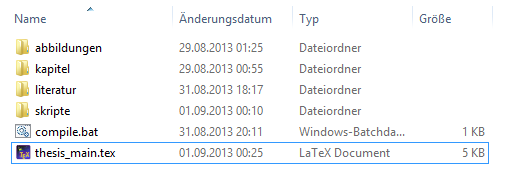
\includegraphics[width=1\textwidth]{verzeichnisStruktur}
% \end{figure}
\end{appendices}
\addtocontents{toc}{\protect\setcounter{tocdepth}{2}}

%-----------------------------------
% Literaturverzeichnis
%-----------------------------------
\newpage

% Die folgende Zeile trägt ALLE Werke aus literatur.bib in das
% Literaturverzeichnis ein, egal ob sie zietiert wurden oder nicht.
% Der Befehl ist also nur zum Test der Skripte sinnvoll und muss bei echten
% Arbeiten entfernt werden.
%\nocite{*}

%\addcontentsline{toc}{section}{Literatur}

% Die folgenden beiden Befehle würden ab dem Literaturverzeichnis wieder eine
% römische Seitennummerierung nutzen.
% Das ist nach dem Leitfaden nicht zu tun. Dort steht nur dass 'sämtliche
% Verzeichnisse VOR dem Textteil' römisch zu nummerieren sind. (vgl. S. 3)
%\pagenumbering{Roman} %Zähler wieder römisch ausgeben
%\setcounter{page}{4}  %Zähler manuell hochsetzen

% Ausgabe des Literaturverzeichnisses

% Keine Trennung der Werke im Literaturverzeichnis nach ihrer Art
% (Online/nicht-Online)
%\begin{RaggedRight}
%\printbibliography
%\end{RaggedRight}

% Alternative Darstellung, die laut Leitfaden genutzt werden sollte.
% Dazu die Zeilen auskommentieren und folgenden code verwenden:

% Literaturverzeichnis getrennt nach Nicht-Online-Werken und Online-Werken
% (Internetquellen).
% Die Option nottype=online nimmt alles, was kein Online-Werk ist.
% Die Option heading=bibintoc sorgt dafür, dass das Literaturverzeichnis im
% Inhaltsverzeichnis steht.
% Es ist übrigens auch möglich mehrere type- bzw. nottype-Optionen anzugeben, um
% noch weitere Arten von Zusammenfassungen eines Literaturverzeichnisse zu
% erzeugen.
% Beispiel: [type=book,type=article]
\printbibliography[nottype=online,heading=bibintoc,title={\langde{Literaturverzeichnis}\langen{Bibliography}}]

% neue Seite für Internetquellen-Verzeichnis
\newpage

% Laut Leitfaden 2018, S. 14, Fussnote 44 stehen die Internetquellen NICHT im
% Inhaltsverzeichnis, sondern gehören zum Literaturverzeichnis.
% Die Option heading=bibintoc würde die Internetquelle als eigenen Eintrag im
% Inhaltsverzeicnis anzeigen.
%\printbibliography[type=online,heading=bibintoc,title={\headingNameInternetSources}]
\printbibliography[type=online,heading=subbibliography,title={\headingNameInternetSources}]

\newpage
\pagenumbering{gobble} % Keine Seitenzahlen mehr

%-----------------------------------
% Ehrenwörtliche Erklärung
%-----------------------------------
\section*{%
	\langde{Ehrenwörtliche Erklärung}
	\langen{Declaration in lieu of oath}}
\langde{Hiermit versichere ich, dass ich die angemeldete Prüfungsleistung in allen Teilen ei-
genständig ohne Hilfe von Dritten anfertigen und keine anderen als die in der Prüfungs-
leistung angegebenen Quellen und zugelassenen Hilfsmittel verwenden werde. Sämt-
liche wörtlichen und sinngemäßen Übernahmen inklusive KI-generierter Inhalte werde
ich kenntlich machen.

Diese Prüfungsleistung hat zum Zeitpunkt der Abgabe weder in gleicher noch in ähn-
licher Form, auch nicht auszugsweise, bereits einer Prüfungsbehörde zur Prüfung vor-
gelegen; hiervon ausgenommen sind Prüfungsleistungen, für die in der Modulbeschrei-
bung ausdrücklich andere Regelungen festgelegt sind.

Mir ist bekannt, dass die Zuwiderhandlung gegen den Inhalt dieser Erklärung einen
Täuschungsversuch darstellt, der das Nichtbestehen der Prüfung zur Folge hat und da-
neben strafrechtlich gem. § 156 StGB verfolgt werden kann. Darüber hinaus ist mir
bekannt, dass ich bei schwerwiegender Täuschung exmatrikuliert und mit einer Geld-
buße bis zu 50.000 EUR nach der für mich gültigen Rahmenprüfungsordnung belegt
werden kann.  

Ich erkläre mich damit einverstanden, dass diese Prüfungsleistung zwecks Plagiatsprü-
fung auf die Server externer Anbieter hochgeladen werden darf. Die Plagiatsprüfung
stellt keine Zurverfügungstellung für die Öffentlichkeit dar.
}
\langen{I hereby declare that I produced the submitted paper with no assistance from any other party and without the use of any unauthorized aids and, in particular, that I have marked as quotations all passages which are reproduced verbatim or near-verbatim from publications. Also, I declare that the submitted print version of this thesis is identical with its digital version. Further, I declare that this thesis has never been submitted before to any examination board in either its present form or in any other similar version. I herewith \textcolor{red}{agree/disagree} that this thesis may be published. I herewith consent that this thesis may be uploaded to the server of external contractors for the purpose of submitting it to the contractors’ plagiarism detection systems. Uploading this thesis for the purpose of submitting it to plagiarism detection systems is not a form of publication.}


\par\medskip
\par\medskip

\vspace{5cm}

\begin{table}[H]
	\centering
	\begin{tabular*}{\textwidth}{c @{\extracolsep{\fill}} ccccc}
		\myOrt, \the\day.\the\month.\the\year
		&
		% Hinterlege deine eingescannte Unterschrift im Verzeichnis /abbildungen und nenne sie unterschrift.png
		% Bilder mit transparentem Hintergrund können teils zu Problemen führen
		
\includegraphics[width=0.35\textwidth]{unterschrift}\vspace*{-0.35cm}
		\\
		\rule[0.5ex]{12em}{0.55pt} & \rule[0.5ex]{12em}{0.55pt} \\
		\langde{(Ort, Datum)}\langen{(Location, Date)} & \langde{(Eigenhändige Unterschrift)}\langen{(handwritten signature)}
		\\
	\end{tabular*} \\
\end{table}

\end{document}
